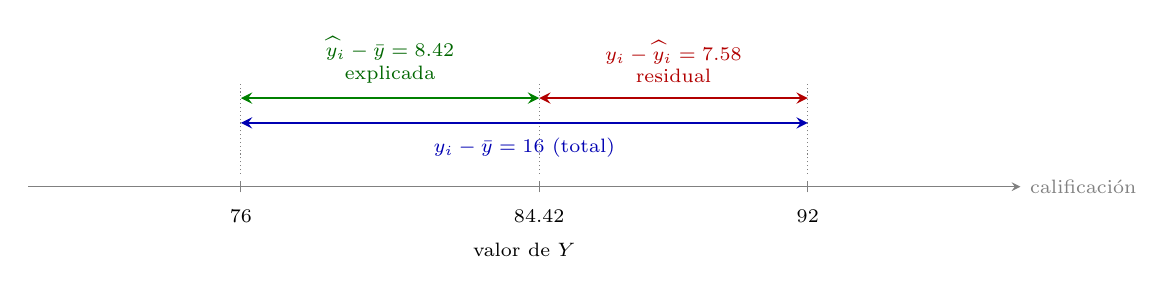
\begin{tikzpicture}[x=0.45cm,y=0.9cm,>=stealth,font=\scriptsize]
    % Para el estudiante 5: media 76, ajuste 84.42 y respuesta observada 92.
    \draw[->,gray] (70,0) -- (98,0) node[right] {calificación};
    \foreach \x/\etiqueta in {76/76,84.42/84.42,92/92} {
        \draw[gray] (\x,-0.08) -- (\x,0.08);
        \node[below=3pt] at (\x,-0.08) {\etiqueta};
    }
    \node[below=17pt,align=center] at (84,0) {valor de $Y$};

    \draw[densely dotted,gray] (76,0.18) -- (76,1.45);
    \draw[densely dotted,gray] (84.42,0.18) -- (84.42,1.45);
    \draw[densely dotted,gray] (92,0.18) -- (92,1.45);

    \draw[<->,thick,green!50!black] (76,1.25) -- (84.42,1.25);
    \node[above=2pt,align=center,text=green!40!black] at (80.21,1.25)
        {$\widehat y_i-\bar y=8.42$\\explicada};
    \draw[<->,thick,red!70!black] (84.42,1.25) -- (92,1.25);
    \node[above=2pt,align=center,text=red!70!black] at (88.21,1.25)
        {$y_i-\widehat y_i=7.58$\\residual};

    \draw[<->,thick,blue!70!black] (76,0.9) -- (92,0.9);
    \node[below=2pt,align=center,text=blue!70!black] at (84,0.9)
        {$y_i-\bar y=16$ (total)};
\end{tikzpicture}